\documentclass[preview]{standalone}

\usepackage{amsmath}
\usepackage{amssymb}
\usepackage{stellar}
\usepackage{definitions}
\usepackage{tikz}

\begin{document}

\id{topology-definitions-exercises}
\genpage

\section{Exercises}

\begin{snippetexercise}{topology-classification-ex-1}{}
    Consider the \set
    \[
        E = \left\{
            x_n = \frac{1}{n} \ \middle|\ n \in \naturalnumbers^\exceptzero
        \right\}
        \cup (2,3) \cup \{4\}
    \]
    Characterize the various types of points in the standard topology for the real line.
\end{snippetexercise}

\begin{snippetsolution}{topology-classification-ex-1-sol}{}
    \begin{center}
    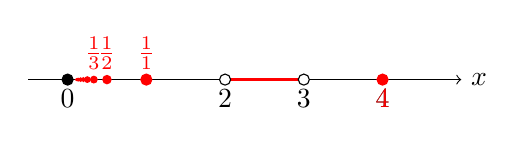
\begin{tikzpicture}

        % Axis
        \draw[->] (-0.5,0) -- (5,0) node[right] {$x$};
        
        % Points for 1/n
        \draw[fill=red, red] ({1/1},0) circle (2pt) node[above] {$\frac{1}{1}$};
        \draw[fill=red, red] ({1/2},0) circle (1.5pt) node[above] {$\frac{1}{2}$};
        \draw[fill=red, red] ({1/3},0) circle (1.2pt) node[above] {$\frac{1}{3}$};
        \draw[fill=red, red] ({1/4},0) circle (1.0pt);
        \draw[fill=red, red] ({1/5},0) circle (0.7pt);
        \draw[fill=red, red] ({1/6},0) circle (0.6pt);
        \draw[fill=red, red] ({1/7},0) circle (0.5pt);
        \draw[fill=red, red] ({1/8},0) circle (0.4pt);
        \draw[fill=red, red] ({1/9},0) circle (0.3pt);

        \node[below] at (2,0) {$2$};
        \node[below] at (3,0) {$3$};
        \node[below] at (4,0) {$4$};

        \draw[thick, red, fill=red] (2,0) -- (3,0);
        \draw[fill=black] (0,0) circle (2pt) node[below] {\(0\)};
        \draw[fill=red, red] (4,0) circle (2pt) node[below] {\(4\)};
        \draw[fill=white] (2,0) circle (2pt); % Open circle at 2
        \draw[fill=white] (3,0) circle (2pt); % Open circle at 3
    \end{tikzpicture}
    \end{center}
    \begin{itemize}
        \item the \set \((2,3)\) is comprised of \interiorpoint[interior points]
        as there exist \(r = \min\{3-x,x-2\}\), where clearly \((x-r, x+r) \subseteq E\);
        \item the \boundarypoint[boundary points] are \(2,3,4\) and all the points of the form \(\frac{1}{n}\) for \(n\in\naturalnumbers^\exceptzero\).
        The point \(0\) is also a \boundarypoint;
        \item the isolated points are the ones of the form \(\frac{1}{n}\) for \(n\in\naturalnumbers^\exceptzero\) and \(4\).
        \item the \exteriorpoint[exterior points] are
        \[ (1,2) \cup (4,+\infty) \cup (-\infty, 0) \cup \bigcup_{n=1}^\infty \left( \frac{1}{n+1}, \frac{1}{n} \right) \]
        \item the \accumulationpoint[accumulation points] are the ones in \([2,3] \cup \{0\}\).
    \end{itemize}
\end{snippetsolution}

\end{document}